% !TEX root = knottedMain.tex
\documentclass[varwidth=\maxdimen]{standalone}

\usepackage{mathtools,amssymb,mathrsfs,dutchcal,upgreek,faktor,accents,etoolbox,multicol}
\usepackage[dvipsnames]{xcolor}
\definecolor{mygreen}{RGB}{	8,156,79 }
\usepackage{tikz,tikz-cd}
\usetikzlibrary{patterns,knots,arrows.meta,decorations.markings}
\tikzset{>={Straight Barb[scale=0.85]}}
\tikzcdset{
  cells={font=\everymath\expandafter{\the\everymath\displaystyle}},
  arrow style=tikz,
  diagrams={>={Straight Barb[scale=0.85]}},
  every label/.append style = {font = \small}
}


\begin{document}

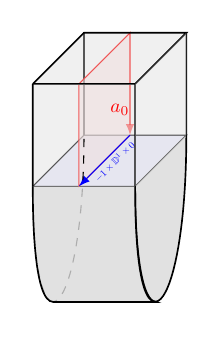
\begin{tikzpicture}[scale=1.3,every node/.style={scale=0.7}]
\clip (-0.8,-2) rectangle (0.8,0.8);
    \draw
        (-0.25,-0.25) rectangle (0.75,0.75);
    \fill[blue!10,fill opacity=0.6,draw=black]
        (-0.75,-0.75) -- (0.25,-0.75) -- 
        (0.75,-0.25) -- (-0.25,-0.25) -- (-0.75,-0.75);
    \fill[red!10,fill opacity=0.6,draw=red,-latex]
          (0.2,-0.25) -- (-0.3,-0.75) -- (-0.3,0.25) --
         (0.2,0.75) -- (0.2,-0.25);
    \fill[black!15,fill opacity=0.4,draw=black,semithick]
        (-0.75,0.25) -- (0.25,0.25) -- 
        (0.75,0.75) -- (-0.25,0.75) -- (-0.75,0.25);

    \fill[black!15,fill opacity=0.4] (-0.75,-0.75) rectangle (0.25,0.25);

    \draw  (0.1,0) node[red]{$a_0$};
    \draw[blue,-latex] (0.2,-0.25) -- (-0.3,-0.75) node[right,pos=0.4,below,scale=0.5,rotate=45]{$-1\times\mathbb{D}^1\times0\,$}; 

    \fill[black!15,fill opacity=0.8]
        (0.25,-0.75) to[out=-90,in=-90,distance =1.8cm] (0.75,-0.25)
        -- (0.25,-0.75);
    \draw[semithick]
        (-0.75,-0.75) -- (-0.75,0.25) 
        (0.25,0.25) -- (0.25,-0.75) to[out=-90,in=-90,distance =1.8cm] (0.75,-0.25) -- (0.75,0.75);
    \draw[dashed]
        (-0.75,-0.75) to[out=-90,in=-90,distance =1.8cm] (-0.25,-0.25);
     \fill[black!15,fill opacity=0.8]
        (-0.75,-0.75) to[out=-90,in=-180,distance =0.2cm] (-0.55,-1.88)
        -- (0.45,-1.88) to[in=-90,out=-180,distance =0.2cm] (0.25,-0.75) 
        -- (-0.75,-0.75);
     \draw[semithick]
        (-0.75,-0.75) to[out=-90,in=-180,distance =0.2cm] (-0.55,-1.88)
        -- (0.45,-1.88) to[in=-90,out=-180,distance =0.2cm] (0.25,-0.75) 
        ;
    \fill[black!15,fill opacity=0.4]
        (0.25,0.25) -- (0.25,-0.75) -- (0.75,-0.25) -- (0.75,0.75) --(0.25,0.25) ;

\end{tikzpicture}
\end{document}